\documentclass[12pt,a4paper]{article}
\usepackage{task}

\newcommand{\contestName}{MateInfoUB}
\newcommand{\contestDates}{18 Mai 2025}
\newcommand{\contestPlace}{Facultatea de Matematic\v a-Informatic\v a}
\newcommand{\contestRound}{Runda Final\v a}
%\newcommand{\contestRound}{Rund\v a de Test}
\newcommand{\statementLanguage}{Rom\^ an\v a (Oficial)}
\newcommand{\taskShortName}{Vârcolaci}


\definecolor{Brown}{cmyk}{0,0.81,1,0.60}
\definecolor{OliveGreen}{cmyk}{0.64,0,0.95,0.40}
\definecolor{CadetBlue}{cmyk}{0.62,0.57,0.23,0}
\definecolor{lightlightgray}{gray}{0.9}

\lstset{
% language=C++,                             % Code langugage
basicstyle=\ttfamily,                   % Code font, Examples: \footnotesize, \ttfamily
keywordstyle=\bfseries,        % Keywords font ('*' = uppercase)
commentstyle=\color{gray},              % Comments font
columns=flexible,
% numbers=left,                           % Line nums position
% numberstyle=\tiny,                      % Line-numbers fonts
% stepnumber=1,                           % Step between two line-numbers
% numbersep=5pt,                          % How far are line-numbers from code
% backgroundcolor=\color{lightlightgray}, % Choose background color
% frame=none,                             % A frame around the code
% tabsize=2,                              % Default tab size
% captionpos=b,                           % Caption-position = bottom
% breaklines=true,                        % Automatic line breaking?
% breakatwhitespace=false,                % Automatic breaks only at whitespace?
% showspaces=false,                       % Dont make spaces visible
% showtabs=true,                         % Dont make tabls visible
}


\setlength{\parskip}{0pt}

\begin{document}
% Tex fragment for task statement headers
% Usage:
%       % Defining parameters required for header
%       \newcommand{\contestName}{Name of the Contest Series}
%       \newcommand{\contestDates}{Month 1 -- 8 20XX}
%       \newcommand{\contestPlace}{City, Country}
%       \newcommand{\contestRound}{Day 1}
%       \newcommand{\statementLanguage}{en (US)}
%       \newcommand{\taskShortName}{task_short_name}
%       % Tex fragment for task statement headers
% Usage:
%       % Defining parameters required for header
%       \newcommand{\contestName}{Name of the Contest Series}
%       \newcommand{\contestDates}{Month 1 -- 8 20XX}
%       \newcommand{\contestPlace}{City, Country}
%       \newcommand{\contestRound}{Day 1}
%       \newcommand{\statementLanguage}{en (US)}
%       \newcommand{\taskShortName}{task_short_name}
%       % Tex fragment for task statement headers
% Usage:
%       % Defining parameters required for header
%       \newcommand{\contestName}{Name of the Contest Series}
%       \newcommand{\contestDates}{Month 1 -- 8 20XX}
%       \newcommand{\contestPlace}{City, Country}
%       \newcommand{\contestRound}{Day 1}
%       \newcommand{\statementLanguage}{en (US)}
%       \newcommand{\taskShortName}{task_short_name}
%       \input{header.tex}
%


%--------------------- tools ----------------------
\makeatletter
% \expandafter for the case that the parameter is given in a command
\newcommand{\escapeUnderscores}[1]{\expandafter\@repl@underscores#1_\relax}
\def\@repl@underscores#1_#2\relax{%
    \ifx \relax #2\relax
        % #2 is empty => finish
        #1%
    \else
        % #2 is not empty => underscore was contained, needs to be replaced
        #1%
        \textunderscore
        % continue replacing
        % #2 ends with an extra underscore so I don't need to add another one
        \@repl@underscores#2\relax
    \fi
}
\makeatother
% -------------------------------------------------

\vspace*{-3em}\hspace*{-.5cm}
\begin{tabular}{ccl}
    \hspace{1mm}
\includegraphics[width=2.2cm,valign=b]{logo.jpeg}
    & 
    \begin{minipage}[b]{10cm}
        \setlength{\baselineskip}{1.05\baselineskip}
        \sffamily
        \makebox[0pt][l]{\bfseries \large \contestName}  \\
        \contestDates \\ 
        \contestPlace
    \end{minipage}
    & 
    \begin{minipage}[b]{3.7cm}
        \begin{flushright}
            \makebox[0pt][r]{\ttfamily \bfseries \large \escapeUnderscores{\taskShortName}}  \\[.2em]
            \sffamily
            \contestRound \\
            \statementLanguage
        \end{flushright}
    \end{minipage}
\end{tabular} 
\hrule height .06em
%


%--------------------- tools ----------------------
\makeatletter
% \expandafter for the case that the parameter is given in a command
\newcommand{\escapeUnderscores}[1]{\expandafter\@repl@underscores#1_\relax}
\def\@repl@underscores#1_#2\relax{%
    \ifx \relax #2\relax
        % #2 is empty => finish
        #1%
    \else
        % #2 is not empty => underscore was contained, needs to be replaced
        #1%
        \textunderscore
        % continue replacing
        % #2 ends with an extra underscore so I don't need to add another one
        \@repl@underscores#2\relax
    \fi
}
\makeatother
% -------------------------------------------------

\vspace*{-3em}\hspace*{-.5cm}
\begin{tabular}{ccl}
    \hspace{1mm}
\includegraphics[width=2.2cm,valign=b]{logo.jpeg}
    & 
    \begin{minipage}[b]{10cm}
        \setlength{\baselineskip}{1.05\baselineskip}
        \sffamily
        \makebox[0pt][l]{\bfseries \large \contestName}  \\
        \contestDates \\ 
        \contestPlace
    \end{minipage}
    & 
    \begin{minipage}[b]{3.7cm}
        \begin{flushright}
            \makebox[0pt][r]{\ttfamily \bfseries \large \escapeUnderscores{\taskShortName}}  \\[.2em]
            \sffamily
            \contestRound \\
            \statementLanguage
        \end{flushright}
    \end{minipage}
\end{tabular} 
\hrule height .06em
%


%--------------------- tools ----------------------
\makeatletter
% \expandafter for the case that the parameter is given in a command
\newcommand{\escapeUnderscores}[1]{\expandafter\@repl@underscores#1_\relax}
\def\@repl@underscores#1_#2\relax{%
    \ifx \relax #2\relax
        % #2 is empty => finish
        #1%
    \else
        % #2 is not empty => underscore was contained, needs to be replaced
        #1%
        \textunderscore
        % continue replacing
        % #2 ends with an extra underscore so I don't need to add another one
        \@repl@underscores#2\relax
    \fi
}
\makeatother
% -------------------------------------------------

\vspace*{-3em}\hspace*{-.5cm}
\begin{tabular}{ccl}
    \hspace{1mm}
\includegraphics[width=2.2cm,valign=b]{logo.jpeg}
    & 
    \begin{minipage}[b]{10cm}
        \setlength{\baselineskip}{1.05\baselineskip}
        \sffamily
        \makebox[0pt][l]{\bfseries \large \contestName}  \\
        \contestDates \\ 
        \contestPlace
    \end{minipage}
    & 
    \begin{minipage}[b]{3.7cm}
        \begin{flushright}
            \makebox[0pt][r]{\ttfamily \bfseries \large \escapeUnderscores{\taskShortName}}  \\[.2em]
            \sffamily
            \contestRound \\
            \statementLanguage
        \end{flushright}
    \end{minipage}
\end{tabular} 
\hrule height .06em

\section*{Creaturi 1: Vârcolaci}


\begin{center}
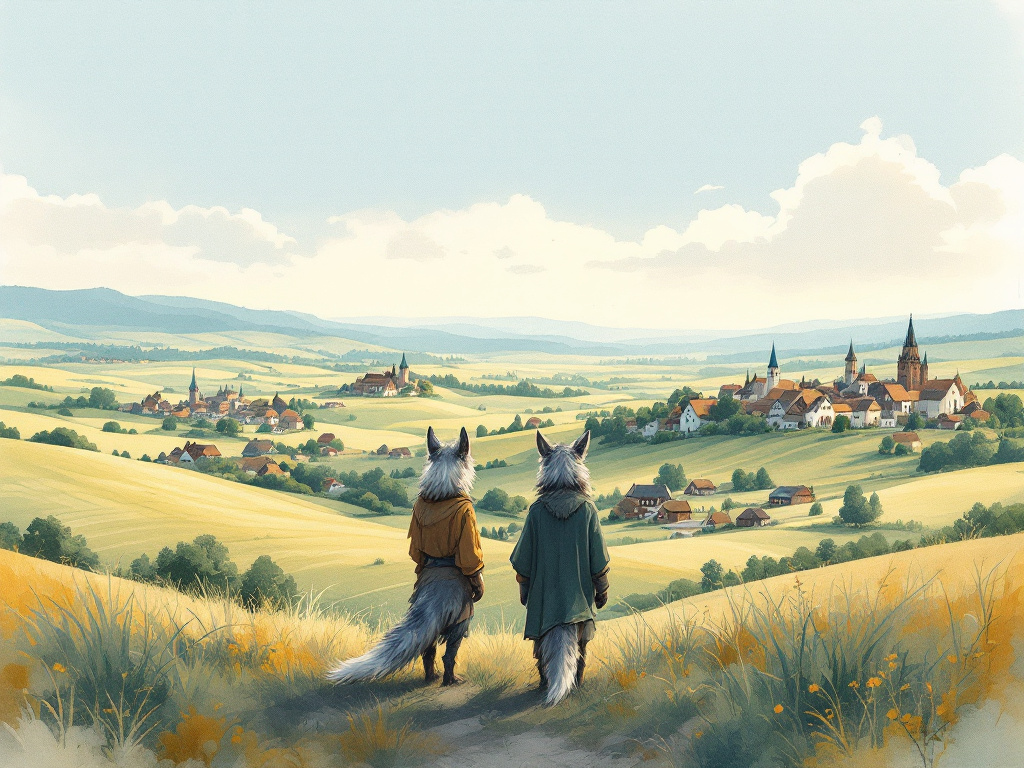
\includegraphics[scale=0.2]{varcolaci.jpg}
\end{center}

Radu și Mircea, doi vârcolaci iscusiți, tocmai au descoperit o vale ascunsă în inima Carpaților, cu sate pline de săteni fragezi și numai buni de mâncat.

\vspace{1em}

În total, cei doi au găsit $N$ sate, satul $i$ având o populație $P_i$ de oameni. Alternativ, fiecare dintre cei doi vârcolaci va ataca câte un sat și va mânca toți sătenii, începând cu Radu. Altfel spus, Radu va ataca un sat, Mircea va ataca alt sat, Radu va ataca alt sat din nou, până când toate satele au fost atacate.

\vspace{1em}

Numerele pare aduc ghinion, așa că fiecare din cei doi dorește să mănânce un număr impar de oameni. Dacă ambii mănâncă un număr par sau ambii mănâncă un număr impar de oameni, atunci sunt la fel de norocoși. Altfel, cel care a mâncat un număr impar de oameni este norocos, și celălalt ghinionist.

\vspace{1em}

Știind că ambii vârcolaci atacă satele în mod optim, cine este norocos? Cei doi nu sunt siguri de valorile lui $P$, așa că vă roagă să rezolvați mai multe scenarii posibile.

\subsection*{Date de intrare}

Pe prima linie se află numărul $T$ de scenarii, urmat de fiecare scenariu, pe câte două linii.

Pe prima linie a fiecărui scenariu, se află numărul $N$, numărul de sate.
Pe a doua linie se află numerele $P_1, P_2, \dots, P_N$.

\subsection*{Date de ieșire}

Afișați răspunsul pentru fiecare scenariu pe câte o linie.

Dacă ambii sunt la fel de norocoși, atunci afișați \textit{"egalitate"}. Altfel, afișați numele celui mai norocos dintre cei doi.

\subsection*{Constrângeri}

\begin{itemize}
    \item $1 \leq T \leq 10$.
    \item $1 \leq N \leq 10^5$.
    \item $1 \leq P_i \leq 10^9 \ \ \forall 1 \leq i \leq N$.
\end{itemize}


\subsection*{Subtask-uri}

\begin{enumerate}
    \item ($20$ de puncte) $N \leq 10, 1 \leq P_i \leq 100 \ \ \forall 1 \leq i \leq N$.
    \item ($20$ de puncte) $N \leq 15$.
    \item ($20$ de puncte) $N \leq 1000$.
    \item ($20$ de puncte) $N \leq 10^4$.
    \item ($20$ de puncte) Nicio constrângere suplimentară.
\end{enumerate}

\subsection*{Exemplu}

\begin{tabular}{|@{}p{0.5\textwidth}@{}|@{}p{0.5\textwidth}@{}|}
\hline
\multicolumn{1}{|c|}{\bfseries Input Standard (\textit{cin})} &
\multicolumn{1}{c|}{\bfseries Output Standard (\textit{cout})} \\
\hline
\begin{textQuoteCell}
3
5
7 2 3 8 1
5
9 2 6 5 6
5
1 10 8 6 6
\end{textQuoteCell} &
\begin{textQuoteCell}
Mircea
egalitate
Radu
\end{textQuoteCell} \\    
\hline
\end{tabular}
\vspace{1em}

\end{document}